\documentclass[../main.tex]{subfiles}
\usepackage{slashed}
\usepackage[table]{xcolor}
\usepackage{hhline}
\usepackage{lipsum}

\let\Bbbk\relax
\usepackage{amsmath}
\usepackage{amsfonts}
\usepackage{simpler-wick}

\begin{document}
\setchapterimage[6.5cm]{images_ch3/...}
\setchapterpreamble[u]{\margintoc}
\chapter[???]{???\footnotemark[0]}
\labch{???}
\fboxsep =1pt % separazione per i box

\section{}
\section{}


\section{Il Momento Magnetico Anomalo}
Riprendiamo l'espressione trovata per il fattore di forma magnetico\footnote{Ricordiamo che, per quanto riportato in equazione (\ref{eq:formfactors_treelevel}), \(F_{2, \text{TREE}}(q^2) = 0\), quindi siamo interessati direttamente al termine ad un loop.} dall'equazione (\ref{eq:formfactor2_final}), ora reinterpretata in termine dei parametri rinormalizzati:
\[
\begin{aligned}
    F_{2,\text{1-loop}}&(q^2) = 2ie^2\int dxdydz \,\delta(x+y+z-1) \int \frac{d^\mathsf d l}{(2\pi)^\mathsf d} \frac{\mathscr{N}_2}{(l^2-\Delta+i\varepsilon)^3}\\
    \text{con }&\mathscr{N}_2 = 2m^2(1-z)\bigl[ 2z + (4-\mathsf d)(1-z) \bigr]\\
    \text{e }& \Delta = (1-z)^2m^2 -xyq^2
\end{aligned}
\]

Quello che ci interessa fare a questo punto è calcolare il valore di integrale quando \(q^2=0\); le ragioni fisiche di questa scelta saranno chiare a breve.

Inoltre, per i motivi discussi durante il calcolo del vertice di interazione ad un loop, questo integrale non è divergente nel regime UV\footnote{Difatti la divergenza ultravioletta del vertice di interazione di QED deriva unicamente dal fattore di forma elettrico.}, ergo possiamo porre fin da subito \(\mathsf d = 4\), il che implica \(\boxed{\mathscr{N}_2 = 4m^2z(1-z)}\).

Attacchiamo allora l'integrale più interno:
\[
 \int \frac{d^4 l}{(2\pi)^4} \frac{4m^2z(1-z)}{(l^2-\Delta+i\varepsilon)^3} \overset{\star}{=}
\]
Essendo \(\Delta = (1-z)^2m^2 \cancel{-xyq^2} > 0\), per via dell'imposizione di \(q^2=0\), non abbiamo problemi di sorta nell'applicare la nostra cara rotazione di Wick, ottenendo quindi:
\[
\overset{\star}{=}  i\int \frac{d^4 l_E}{(2\pi)^4} \frac{4m^2z(1-z)}{(-1)(l_E^2+\Delta)^3} \overset{\star}{=} 
\]
Abbiamo nuovamente a che fare con un integrale euclideo, che ormai mangiamo a colazione grazie all'equazione (\ref{eq:euclidean_integral_general}), in questo caso applicata con \(n=0, m=3\) e \(\mathsf d =4\). Di conseguenza:

\[
\overset{\star}{=} (-i)4m^2z\frac{1}{(4\pi)^2}\frac{1}{\Delta}\frac{\Gamma(1)\Ccancel[blue]{\Gamma(2)}}{\Ccancel[blue]{\Gamma(2)}\Gamma(3)} = \frac{(-i)4m^2z}{(4\pi)^2}\frac{1}{ (1-z)^2m^2}\frac{1}{2}
\]

In conclusione abbiamo il nostro risultato:
\[
\boxed{\int \frac{d^4 l}{(2\pi)^4} \frac{4m^2z(1-z)}{(l^2-\Delta+i\varepsilon)^3} = \frac{(-i)z}{8\pi^2(1-z)^2}}
\]

A questo punto possiamo procedere con l'integrale principale. Scriviamo:
\begin{align*}
    F_{2,\text{1-loop}}(q^2=0) &= \Ccancel[blue]{2}\Ccancel[red]{i}e^2\int dxdydz \,\delta(x+y+z-1) \frac{\Ccancel[red]{(-i)}z}{\underset{4}{\Ccancel[blue]{8}}\pi^2(1-z)^2}\\
    &=\frac{e^2}{4\pi^2}\int dxdydz \,\delta(x+y+z-1) \frac{z}{(1-z)^2} \overset{\blacklozenge}{=}
\end{align*}

Ora integriamo su $x$ e $y$ usando la $\delta$, i.e.:
\marginnote{Dall'esercizio \ref{ex:1loop_formfactor1}: la $\delta$ ci permettere di togliere una delle variabili, ma dobbiamo ricordarci dei limiti di integrazione! Infatti \[0\leq y\overset{\delta}{=} 1-x-z\leq 1\] implica
\[
\begin{cases}
1-x-z\leq 1\\
1-x-z\geq 0
\end{cases}
\Rightarrow
\begin{cases}
x+z\geq 0\\
x\leq 1-z
\end{cases}
\]}
\[
\int\limits_0^1 dxdy \,\delta(x+y+z-1)=\int\limits_0^{1-z} dx = (1-z)
\]
Possiamo quindi semplificare il denominatore nell'integrale precedente, ottenendo
\[
\overset{\blacklozenge}{=} \frac{e^2}{4\pi^2}\int\limits_0^1 dz \, z
\]

A questo punto il gioco è fatto, integriamo su $z$ e, ricordando la definizione della costante di struttura fine $\alpha = \nicefrac{e^2}{4\pi}$, arriviamo al risultato finale:
\begin{equation}
    \boxed{F_{2,\text{1-loop}}(q^2=0) = \frac{\alpha}{2\pi}}
    \label{eq:F2_q0}
\end{equation}
Tuttavia, per comprendere appieno questo risultato, abbiamo bisogno di una piccola introduzione.

\subsection{Momento giromagnetico dell'elettrone}
\marginnote{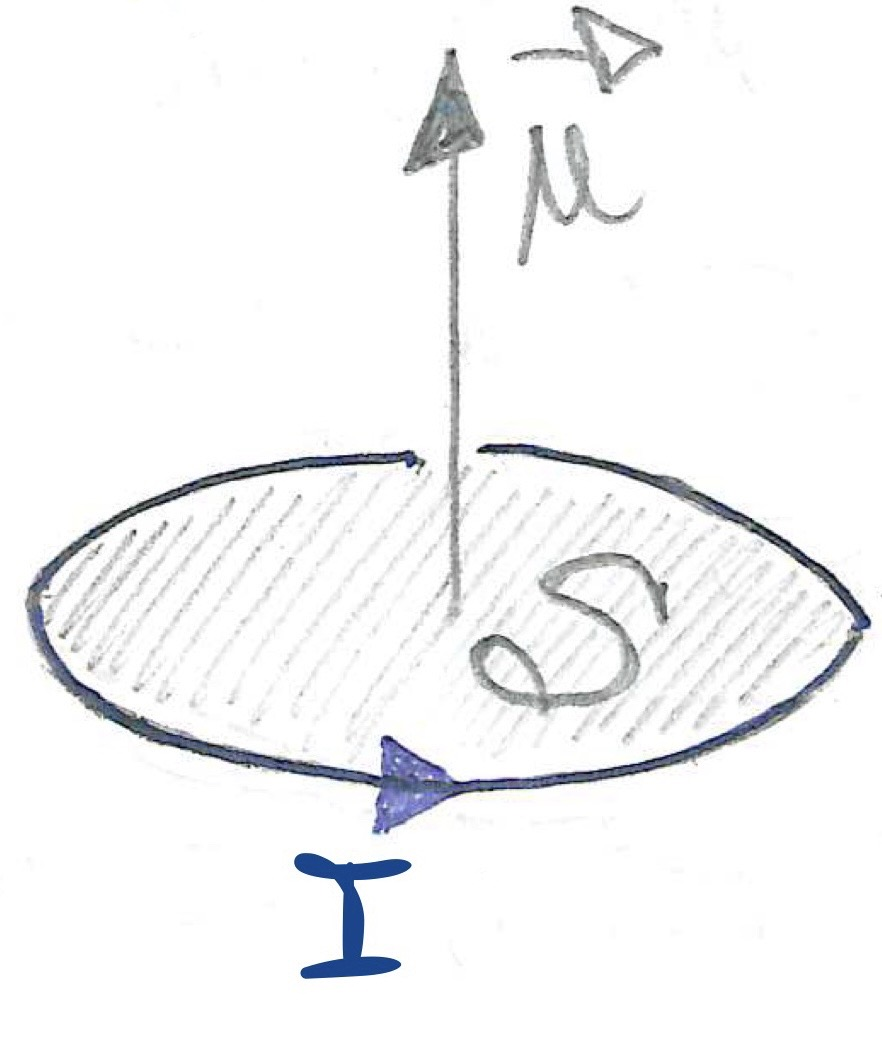
\includegraphics[]{images_ch5/magn_mom.jpg}}
 
\begin{definition}
    \textbf{(Momento Magnetico.)}
    
    Consideriamo una corrente planare di modulo $I$, che racchiude una superficie di area $S$ tale che \(\Vec{S} = S\hat{n}\), come in figura a lato.
    
    Si definisce momento magnetico il vettore 
    \begin{equation}
        \Vec{\mu} = I\Vec{S}
        \label{eq:magn_moment}
    \end{equation}
    Perpendicolare rispetto alla spira percorsa dalla corrente, secondo la regola della mano detra.
\end{definition}

In presenza di un campo magnetico $\Vec{B}$, una spira subisce una coppia data da \(\Vec\tau = \Vec\mu \times \Vec{B} \), e si sviluppa un'energia potenziale associata alla direzione della spira rispetto al campo magnetico, i.e.:
\begin{equation}
    \boxed{U = -\Vec\mu\cdot\Vec{B}}
    \label{eq:potential_energy_magn_mom}
\end{equation}

La configurazione con \(\Vec{\mu}\parallel\Vec{B}\) coincide con la configurazione ad energia potenziale minore.

Consideriamo ora il caso in cui la corrente $I$ è generata da una carica $q$ che si muove nella spira con velocità angolare $\omega$. Tale corrente è esprimibile come segue:
\[
I = \frac{q}{T} = \frac{q\omega}{2\pi}
\]

Di conseguenza, assumendo la spira come circolare, con raggio $a$, abbiamo dalla sua definizione:
\[
\Vec\mu = \frac{q\omega}{2\pi}\pi a^2 \hat{n} = \frac{q}{2m} (\omega m a^2) \hat{n} = \frac{q}{2m}\Vec{L}
\]
dove abbiamo introdotto il momento angolare \(\Vec{L}=(\omega m a^2) \hat{n}\).

Quindi abbiamo:
\[
\boxed{\Vec\mu = \frac{q}{2m}\Vec{L} \quad ; \quad U = -\frac{q}{2m}\Vec{L}\cdot\Vec{B}}
\]

Classicamente, il momento magnetico è proporzionale al momento angolare delle particelle cariche. In meccanica quantistica, questa relazione si generalizza con la presenza dello spin.

Prendendo ad esempio un elettrone a riposo, il momento di dipolo magnetico è fornito dalla relazione:
\begin{equation}
    \boxed{\Vec\mu_e = \frac{-ge}{2m}\Vec{S}}
    \label{eq:electrone_dipole_moment}
\end{equation}
dove $\Vec{S}$ è l'operatore di spin, mentre $g$ è detto \textbf{momento giromagnetico dell'elettrone}.

Inoltre, l'Hamiltoniana di interazione in presenza di un campo magnetico esterno è
\begin{equation}
    \boxed{H_\text{int} = +\frac{ge}{2m}\Vec{S}\cdot\Vec{B}}
    \label{eq:magn_inter_hamiltonian}
\end{equation}


\subsection{Predizione di $g$ in QED}

Vogliamo calcolare il valore del momento giromagnetico dell'elettrone in QED al tree-level. per farlo partiamo nuovamente dallo scattering Coulombiano in presenza di un potenziale esterno statico
\[
\feynmandiagram[vertical'=a to b] {
    i1 -- [fermion, edge label'=\(p\)] a[small, dot] -- [fermion, edge label'=\(p'\)] i2,
    b[large, crossed dot, label=right:\(A_\mu^{\text{ext}}(\Vec{x})\)] -- [photon, momentum'=\(q\)] a
    };
\]
con \(q=p'-p\).

Come già argomentato all'inizio di questo capitolo, si trova:
\[
S_{fi} = (2\pi)\delta(E_{p'}-E_p)(ie)\bar u(p',s)\gamma^\mu u(p,r)A_\mu^{\text{ext}}(\Vec{q})
\]
La differenza rispetto a quanto già visto sta nel fatto che ora associamo ad \(A^\mu\) il 4-potenziale elettromagnetico dovuto ad un campo magnetico, i.e. 
\[
\begin{cases}
A^0=0\\
\Vec{B}=\Vec\nabla\times\Vec{A}
\end{cases}
\] 
In questo caso, la parte dell'ampiezza che sopravvive è quella che concerne la corrente spaziale, ovvero:
\[
\boxed{S_{fi} = (2\pi)\delta(E_{p'}-E_p)(ie)\bar u(p',s)\gamma^i u(p,r)A_i^{\text{ext}}(\Vec{q})}
\]

Ora valutiamone il limite non relativistico, lavorando al primo ordine in \(\Vec{q}\) e imponendo \(\Vec{p}=0\) in modo da poterci concentrare sullo spin.

La cinematica è quindi descritta da:
\[
p^\mu = \big(m, -\nicefrac{\Vec{q}}{2}\big) \quad p'^\mu = \big(m, \nicefrac{\Vec{q}}{2}\big)
\]
mentre possiamo esprimere gli spinori come segue:
\[
u(p,s) = \bigg(\frac{E+m}{2m}\bigg)^{\nicefrac{1}{2}}
\begin{pmatrix} 
\chi(s)\\
\frac{\Vec\sigma\cdot\Vec p}{E+m}\chi(s)
\end{pmatrix}\rightarrow
\begin{pmatrix} 
\chi(s)\\
\frac{-\Vec\sigma\cdot\Vec q}{4m}\chi(s)
\end{pmatrix}
\]

Adesso dobbiamo calcolare esplicitamente la corrente \( u^\dagger(p',s)\gamma^0 \gamma^i u(p,r)\).

Con la notazione di Dirac, abbiamo innanzitutto:
\[
\gamma^0\gamma^i = 
\begin{pmatrix}
    \mathbb 1   &   0\\
            0   &   - \mathbb 1
\end{pmatrix}
\begin{pmatrix}
            0   &   \sigma^i\\
    -\sigma^i   &   0
\end{pmatrix}
=
\begin{pmatrix}
            0   &   \sigma^i\\
    \sigma^i   &   0
\end{pmatrix}
\]
Di conseguenza:
\begin{align*}
    u^\dagger(p',s)\gamma^0 \gamma^i u(p,r) 
    &= 
    \begin{pmatrix} 
        \chi^\dagger(s) & \frac{\Vec\sigma\cdot\Vec q}{4m}\chi^\dagger(s)
    \end{pmatrix}
    \begin{pmatrix} 
        -\sigma^i\frac{\Vec\sigma\cdot\Vec q}{4m}\chi(r)\\
        \sigma^i\chi(r)
    \end{pmatrix}\\
    &=-\frac{1}{4m}\chi^\dagger(s) \big[\sigma^i (\Vec\sigma\cdot\Vec q)\big] \chi(r) + \frac{1}{4m}\chi^\dagger(s) \big[(\Vec\sigma\cdot\Vec q) \sigma^i\big] \chi(r)\\
    &=\frac{1}{4m}\chi^\dagger(s) \big[\sigma^j \sigma^i - \sigma^i \sigma^j\big]q^j \ \chi(r)
\end{align*}
Ricordiamo a questo punto le relazioni di commutazione tra le matrici di Pauli:
\(\big[\sigma^j, \sigma^i\big] = 2i\epsilon^{jik}\sigma^k\) e con un un paio di ulteriori manipolazioni (tra cui in particolare \(\epsilon^{jik} = -\epsilon^{ijk}\)) arriviamo al risultato finale:
\marginnote{Ricordiamo che $S^k$ è l'operatore di spin per il campo di Dirac.}
\begin{equation}
    \bar u(p',s)\gamma^i u(p,r) = \frac{-i}{m}\epsilon^{ijk}q^j \underbrace{\chi^\dagger(s)\frac{\sigma^k}{2}\chi(r)}_{\equiv \langle s|S^k|r\rangle}
    \label{eq:spatial_current}
\end{equation}

Ora possiamo sostituire la corrente nell'espressione per l'ampiezza, riscrivendola come segue:
\marginnote{Risulta utile riscrivere la parte spaziale del 4-potenziale in forma controvariante \(A_i\rightarrow A^i\), il che comporta un cambio di segno cancellato dalla permutazione del simbolo di Levi-Civita \(\epsilon^{ijk}\rightarrow-\epsilon^{kji}\), in modo da poter inserire nell'equazione il campo magnetico.}
\begin{align*}
    S_{fi} &\overset{\text{NR}}{=} (2\pi)\delta(E_{p'}-E_p)(ie)\Big[\frac{-i}{m}\epsilon^{ijk}q^j\langle s|S^k|r\rangle \Big]A_i^\text{ext}(\Vec{q})\\
    &= (2\pi)\delta(E_{p'}-E_p)\Big[\frac{e}{m} \textcolor{Green}{\epsilon^{kji}q^j} \langle s|S^k|r\rangle \Big]\textcolor{Green}{A^{\text{ext},i}(\Vec{q})}
\end{align*}

Ricordiamo che la relazione \(\Vec{B}=\Vec\nabla\times\Vec{A}\) si traduce in \(B^k = \epsilon^{kji}\partial_j A^i\), che nello spazio di Fourier diventa \(B^k = \epsilon^{kji}iq^jA^i\), da cui
\[
{-iB^k} = \textcolor{Green}{\epsilon^{kji}q^jA^i}
\]

Abbiamo quindi finalmente l'ampiezza in QED che cercavamo:
\marginnote{È interessante notare come l'equazione (\ref{eq:CoulombQEDamplitude_NR_treelevel}) ci stia dicendo che per mezzo dell'interazione con il campo magnetico si possono avere transizioni di spin!}
\begin{equation}
    \boxed{S_{fi} \overset{\text{NR}}{=} (2\pi)\delta(E_{p'}-E_p)\frac{(-ie)}{m}B^k\langle s|S^k|r\rangle}
    \label{eq:CoulombQEDamplitude_NR_treelevel}
\end{equation}

A questo punto compariamo quanto appena trovato con l'ampiezza calcolata in meccanica quantistica, utilizzando l'operatore (\ref{eq:magn_inter_hamiltonian})
\[
H_\text{int} = \frac{ge}{2m}\Vec{S}\cdot\Vec{B} =  \frac{ge}{2m}S^kB^k
\]

Abbiamo 
\begin{equation}
    \begin{aligned}
        A\big(|s\rangle\rightarrow|r\rangle\big) &= (2\pi)\delta(E_{p'}-E_p) (-i)\langle s|H_\text{int}|r\rangle \\
        & = (2\pi)\delta(E_{p'}-E_p) \frac{g(-ie)}{2m}\langle s|S^k|r\rangle B^k
    \end{aligned}
    \label{eq:CoulombQMamplitude_NR_treelevel}
\end{equation}
È evidente che il momento giromagnetico dell'elettrone, al tree-level, debba essere 
\begin{equation}
    \boxed{g=2}
    \label{eq:electr_gyromagn_factor_treelevel}
\end{equation}

\subsection{$g$ oltre il tree level}
Includiamo le correzioni al loop nel calcolo fatto in sezione precedente, in particolare le correzioni al vertice, i.e.:
\[
 \bar u(p',s)\big(ie\gamma^\mu\big) u(p,r) \rightarrow \bar u(p',s)ie\Gamma^\mu(p',p) u(p,r)
\]
con, dalla (\ref{eq:vertex_formfactors}): \(\Gamma^\mu(p',p) = F_1(q^2)\gamma^\mu +\frac{i\sigma^{\mu\nu}q_\nu}{2m} F_2(q^2)\).

Dopo il processo di rinormalizzazione (in cui viene cancellato il termine UV-divergente \(F_{1,\text{1-loop}}(0)\) per mezzo del contro-termine \(\delta_1\)) il fattore di forma elettrico ha la seguente struttura:
\[
F_1(q^2) \approx 1+\frac{dF_{1,\text{1-loop}}(q^2)}{dq^2}\bigg|_{q^2=0}q^2 +\cdots
\]
Nel paragrafo precedente ci siamo limitati al tree-level, \(F_1(q^2) = 1\), e abbiamo detto di voler lavorare al prim'ordine in $q$. Di conseguenza, introducendo correzioni al loop non abbiamo bisogno di aggiungere termini dipendenti da \(F_1\) e possiamo concentrarci su \(F_2\):
\[
\boxed{\Gamma^\mu\rightarrow\frac{i\sigma^{\mu\nu}q_\nu}{2m}F_2(q^2=0) \quad , \quad q_\mu=(0,\Vec{q})}
\]

In termini di ampiezza di scattering, la correzione da calcolare è, trascurando il fattore \(2\pi\delta(E_{p'}-E_p)\):
\[
{\Delta S_{fi} = (ie)\bar u(p',s) \frac{i\sigma^{\mu\nu}q_\nu}{2m}F_2(q^2=0) u(p,r)A_\mu^\text{ext}(\Vec{q})} \quad , \quad A_\mu = (0,\Vec{A})
\]
di cui sopravvive solo la parte spaziale, che riportiamo utilizzando la notazione controvariante sia per l'impulso che per il potenziale (abbiamo due segni “$-$” che si elidono a vicenda): 

\begin{equation}
    \boxed{\Delta S_{fi} = \frac{(ie)}{2m}\bar u(p',s) i\sigma^{ij}q^j F_2(q^2=0) u(p,r)A^i}
    \label{eq:Sficorrection_start}
\end{equation}

Calcoliamo esplicitamente il prodotto spinoriale, utilizzando per prima cosa il commutatore tra le gamma di Dirac, con cui si identificano le matrici di Pauli in forma relativistica, \(\sigma_{\mu\nu} = \frac{i}{2}\big[\gamma_\mu,\gamma_\nu\big] \) e sostituendo le gamma stese in notazione di Dirac:
\begin{align*}
    \bar u(p',s) \sigma^{ij} u(p,r) &= \bar u(p',s) \frac{i}{2}\big(\gamma^i\gamma^j-\gamma^j\gamma^i\big) u(p,r) \\
    & = \frac{i}{2}\bar u(p',s) 
    \Bigg[
    \begin{pmatrix}
                0   &   \sigma^i \\
        -\sigma^i   &   0
    \end{pmatrix}
    \begin{pmatrix}
                0   &   \sigma^j \\
        -\sigma^j   &   0
    \end{pmatrix}
    -
    \begin{pmatrix}
                0   &   \sigma^j \\
        -\sigma^j   &   0
    \end{pmatrix}
    \begin{pmatrix}
                0   &   \sigma^i \\
        -\sigma^i   &   0
    \end{pmatrix}
    \Bigg] u(p,r)\\
    & = \frac{i}{2}\bar u(p',s) 
    \begin{pmatrix}
        -\sigma^i\sigma^j +\sigma^j\sigma^i  &   0 \\
        0   &  -\sigma^i\sigma^j +\sigma^j\sigma^i
    \end{pmatrix}u(p,r) \overset{\star}{=}
\end{align*}
Sulla diagonale riconosciamo il commutatore tra matrici di Pauli: \(\big[\sigma^j,\sigma^i\big]=2i\epsilon^{jik}\sigma^k\).

Inoltre, come già ribadito, vogliamo mantenere il calcolo al prim'ordine in $q$, quindi, data la presenza di $q^j$ in \(\Delta S_{fi}\), possiamo trascurare la parte proporzionale a $q$ nell'espressione dello spinore, i.e. prendiamo:
\[
u(p,s) = 
\begin{pmatrix}
    \chi(s)\\
    0
\end{pmatrix}
\]
Questo significa che possiamo trascurare la seconda riga della matrice al centro, in quanto il suo contributo verrà annullato dal prodotto con gli spinori.

In sostanza, otteniamo:
\begin{align*}
    \overset{\star}{=} \frac{i}{2}\chi^\dagger(s)\big( 2i\epsilon^{jik}\sigma^k \big) \chi(r) = -2\epsilon^{jik}\chi^\dagger(s) \frac{\sigma^k}{2} \chi(r) = -2\epsilon^{jik}\langle s | S^k | r \rangle
\end{align*}

Riassumendo:
\begin{equation}
    \boxed{\bar u(p',s) \sigma^{ij} u(p,r) = -2\epsilon^{jik}\langle s | S^k | r \rangle}
    \label{eq:current_correction}
\end{equation}

Sostituiamo quindi la (\ref{eq:current_correction}) nella (\ref{eq:Sficorrection_start}) e troviamo:
\begin{align*}
    \Delta S_{fi} = -\frac{e}{2m} q^j F_2(q^2=0) A^i \big[(-2)\epsilon^{jik}\langle s | S^k | r \rangle\big]
\end{align*}
Permutiamo gli indici del simbolo di Levi-Civita \(\epsilon^{jik}\rightarrow\epsilon^{kji}\) (questa volta la permutazione è pari, quindi non produce nessun “$-$”) e ritroviamo l'espressione del campo magnetico \(-iB^k = \epsilon^{kji}q^jA^i\).
Quindi troviamo:
\begin{equation}
    \boxed{\Delta S_{fi} = \frac{-ie}{m} F_2(q^2=0)  B^k\langle s | S^k | r \rangle}
    \label{eq:Sficorrection_end}
\end{equation}

Possiamo allora scrivere \textbf{l'ampiezza totale}:
\begin{equation}
    \boxed{S_{fi} + \Delta S_{fi} = (2\pi)\delta(E_{p'}-E_p)\frac{-ie}{2m}\Big[ 2 + 2F_2(q^2=0) \Big] B^k\langle s | S^k | r \rangle}
    \label{eq:Sfi_total}
\end{equation}
Non ci resta che comparare la (\ref{eq:Sfi_total}) con la (\ref{eq:CoulombQMamplitude_NR_treelevel}). Imponendo il loro rapporto = 1, troviamo la predizione per il \textbf{fattore giromagnetico dell'elettrone ad un loop}, i.e."
\begin{equation}
    \boxed{g=2\big[1 + F_{2,\text{1-loop}}(q^2=0)\big]}\quad , \text{con } F_{2,\text{1-loop}}(q^2=0) \overset{\ref{eq:F2_q0}}{=} \frac{\alpha}{2\pi}
\end{equation}

Possiamo andare oltre: esplicitando il valore del fattore di forma magnetico troviamo \(g=2+\nicefra{\alpha}{\pi}\); inoltre possiamo dare la seguente definizione:
\begin{definition}
    \textbf{(Momento di dipolo magnetico anomalo dell'elettrone.)}

    Sia $g$ il fattore giromagnetico dell'elettrone a qualunque ordine, si definisce momento magnetico anomalo (di dipolo) il fattore:
    \begin{equation}
        a_e\equiv\frac{g-2}{2} \xrightarrow[]{\substack{\text{@ 1-loop}\\\text{in QED}}} a_e=\frac{\alpha}{2\pi}
        \label{eq:anomalous_magn_mom}
    \end{equation}
\end{definition}

\begin{nota}
    Abbiamo incluso solo un loop nel nostro calcolo. Tenere conto di correzioni con un numero di loop maggiore è piuttosto complesso se si vuole procedere analiticamente, in quanto il numero di diagrammi cresce esponenzialmente all'aumentare del numero di loop considerati.
    
    Inoltre, quando il numero di loop diventa sufficientemente elevato, andrebbe tenuto conto anche delle interazioni forti e deboli, dato che i fotoni possono interagire sia con gli adroni che con i \(W^\pm\).
    
    Ciò nonostante, persone con molta pazienza, tanto tempo libero, poca sanità mentale o, forse, computer sufficientemente potenti hanno calcolato il momento magnetico anomalo per l'elettrone ed il muone fino all'ordine $\alpha^5$.
    
    D'altro canto, sperimentalmente conosciamo queste grandezze fisiche con un'enorme precisione:
    \[
    \begin{cases}
        a_e^\text{exp} = 0.00115965218073(22)\\
        a_\mu^\text{exp} = 0.00116592091(63)
    \end{cases}
    \]
    e c'è una piccola discrepanza nel caso del muone:
    \[
     a_\mu^\text{exp} -  a_\mu^\text{th} \approx(23\pm6) \times 10^{-10}
    \]
    Questa discrepanza potrebbe dipendere da fisica oltre il modello standard, ma potrebbe anche dipendere da un piccolo errore teorico nella modellizzazione delle interazioni tra fotoni ed adroni.
\end{nota}

\end{document}

\begin{figure}[h]
    \centering
    \includegraphics{images/semplicementepanati.png}
    \caption*{}
    \label{fig:my_label}
\end{figure}